\documentclass{beamer}
\usepackage[utf8]{inputenc}
% \usepackage[english]{babel}
\usepackage{hyperref}
\usepackage{graphicx}
\graphicspath{{../../../output/figures/Presentation/}}
\usepackage{wrapfig}
\usepackage{subcaption}
\usepackage{booktabs,bbm}
\usepackage[space]{grffile}
% \usepackage[square,numbers]{natbib}
%\bibliographystyle{unsrtnat}

\makeatletter
\let\@@magyar@captionfix\relax
\makeatother
\newtheorem{defn}[theorem]{Definition}
\DeclareMathOperator*{\argmax}{arg\,max}
\DeclareMathOperator*{\argmin}{arg\,min}
\hypersetup{
    allcolors={}
}

\usetheme{Boadilla}
\usecolortheme{beaver}

\usepackage[
backend=biber,
style=bwl-FU,
sorting=ynt
]{biblatex}
\addbibresource{../../main.bib}

\title[Agricultural Index Insurance]{Agricultural Index Insurance: An Optimization Approach}
\author[José Velarde Morales]{José I. Velarde Morales \and Linwei Xin}
\institute[Chicago Booth]
{

  University of Chicago\\
  Booth School of Business

}


\begin{document}
\beamertemplatenavigationsymbolsempty
\frame{\titlepage}
\section{Introduction}


\subsection*{Project Overview}
\begin{frame}{Project Overview}
 \begin{itemize}
    \setlength\itemsep{1em}   
    % \item Traditionally, contracts are designed to maximize correlation between payouts and losses (\cite{chantarat2013designing}).  %This ignores valuable information about the correlation between zones that affects the cost of insuring the whole portfolio. 
    \item The goal of this project is to improve the design of index insurance contracts. I am particularly interested in the developing country setting.  
    \item The original motivation was to develop a method to simultaneously design contracts for all insured zones, in order to better manage risk. However, upon learning more about the context I realized that the optimization based approach could be an improvement even in the single zone case. 
    \item We develop a method that tries to maximize farmer utility, incorporates different kinds of constraints, and yields interpretable contracts. 
    % \item Our method simultaneously determines the contract parameters for different areas, while taking into account the correlation between the areas, reducing risk for the insurer. 
 \end{itemize}
\end{frame}

\section{Background}
\begin{frame}[noframenumbering, plain]
    \frametitle{Content}
    \tableofcontents[currentsection]
  \end{frame}
\subsection{Index Insurance Background}

\begin{frame}{Index Insurance: Definition and Parameters}
\begin{itemize}
    \setlength\itemsep{1em}
    \item Index insurance uses a signal, $\theta$, to predict agricultural loss, $\hat{\ell}(\theta)$
    \item Contract form: $I(\theta) = \min \left \{ \max \left \{a\hat{\ell}(\theta) - b,0 \right \}, 1 \right \}$, $a,b$ are the contract parameters.
    % \item Expected cost for insurer: $C(I(\theta)) = \mathbb{E}[I(\theta)] + c_{\kappa} K(I(\theta))$, where $c_{\kappa}$ is the cost of capital, and $K$ is required capital.
    % \item $K(I(\theta)) = CVaR_{1-\epsilon_P}\left ( I(\theta) \right ) - \mathbb{E}[I(\theta)]$.
\end{itemize}
\end{frame}

\begin{frame}{Example of Index Insurance Contract}
    \begin{figure}
        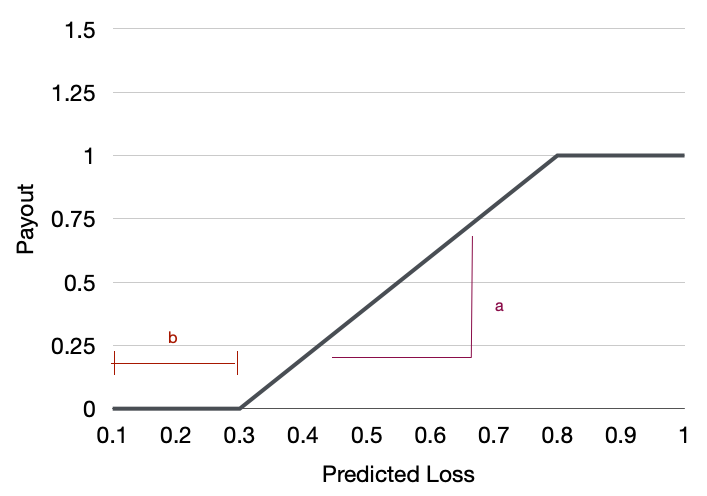
\includegraphics[width=0.9\textwidth]{../../../output/figures/Presentation/sample_insurance_contract.png}
    \end{figure}
\end{frame}

\begin{frame}{Current Methods: Chen}
    \begin{itemize}
        \setlength\itemsep{1em}
        \item NN based approach, end-to-end, directly maps weather variables to payouts. 
        \item \textbf{Pros:} directly maximizes utility, admits price constraints
        \item \textbf{Cons:} not interpretable, hard to adjust
    \end{itemize}
    \end{frame}

\begin{frame}{Current Methods: Kenya ILRB}
    \begin{itemize}
        \setlength\itemsep{1em}
        \item Choose strike value that maximizes correlation between losses and payouts  
        \item \textbf{Pros:} simple, interpretable
        \item \textbf{Cons:} does not admit price constraints. 
    \end{itemize}
    \end{frame}


\section{Optimization Approach}
\begin{frame}[noframenumbering, plain]
    \frametitle{Content}
    \tableofcontents[currentsection]
  \end{frame}

  \begin{frame}{Overview}
    \begin{itemize}
        \setlength\itemsep{2em}
        \item We opt for a "predict-then-optimize" approach. We first train prediction models then design optimal contracts. 
        % \item We use specialized time-series feature extraction algorithms for feature extraction and traditional ML algorithms (e.g. Random Forest, Gradient Boosting, Support Vector Machines)
        % \item These algorithms require less data to train than a neural network approach.
        \item \textbf{Pros:} interpretable results, maximizes utility, admits constraints.
        \item \textbf{Cons:} can overfit if there's insufficient data. 
    \end{itemize}
\end{frame}

\begin{frame}{Our Method Flowchart}
    \begin{figure}
        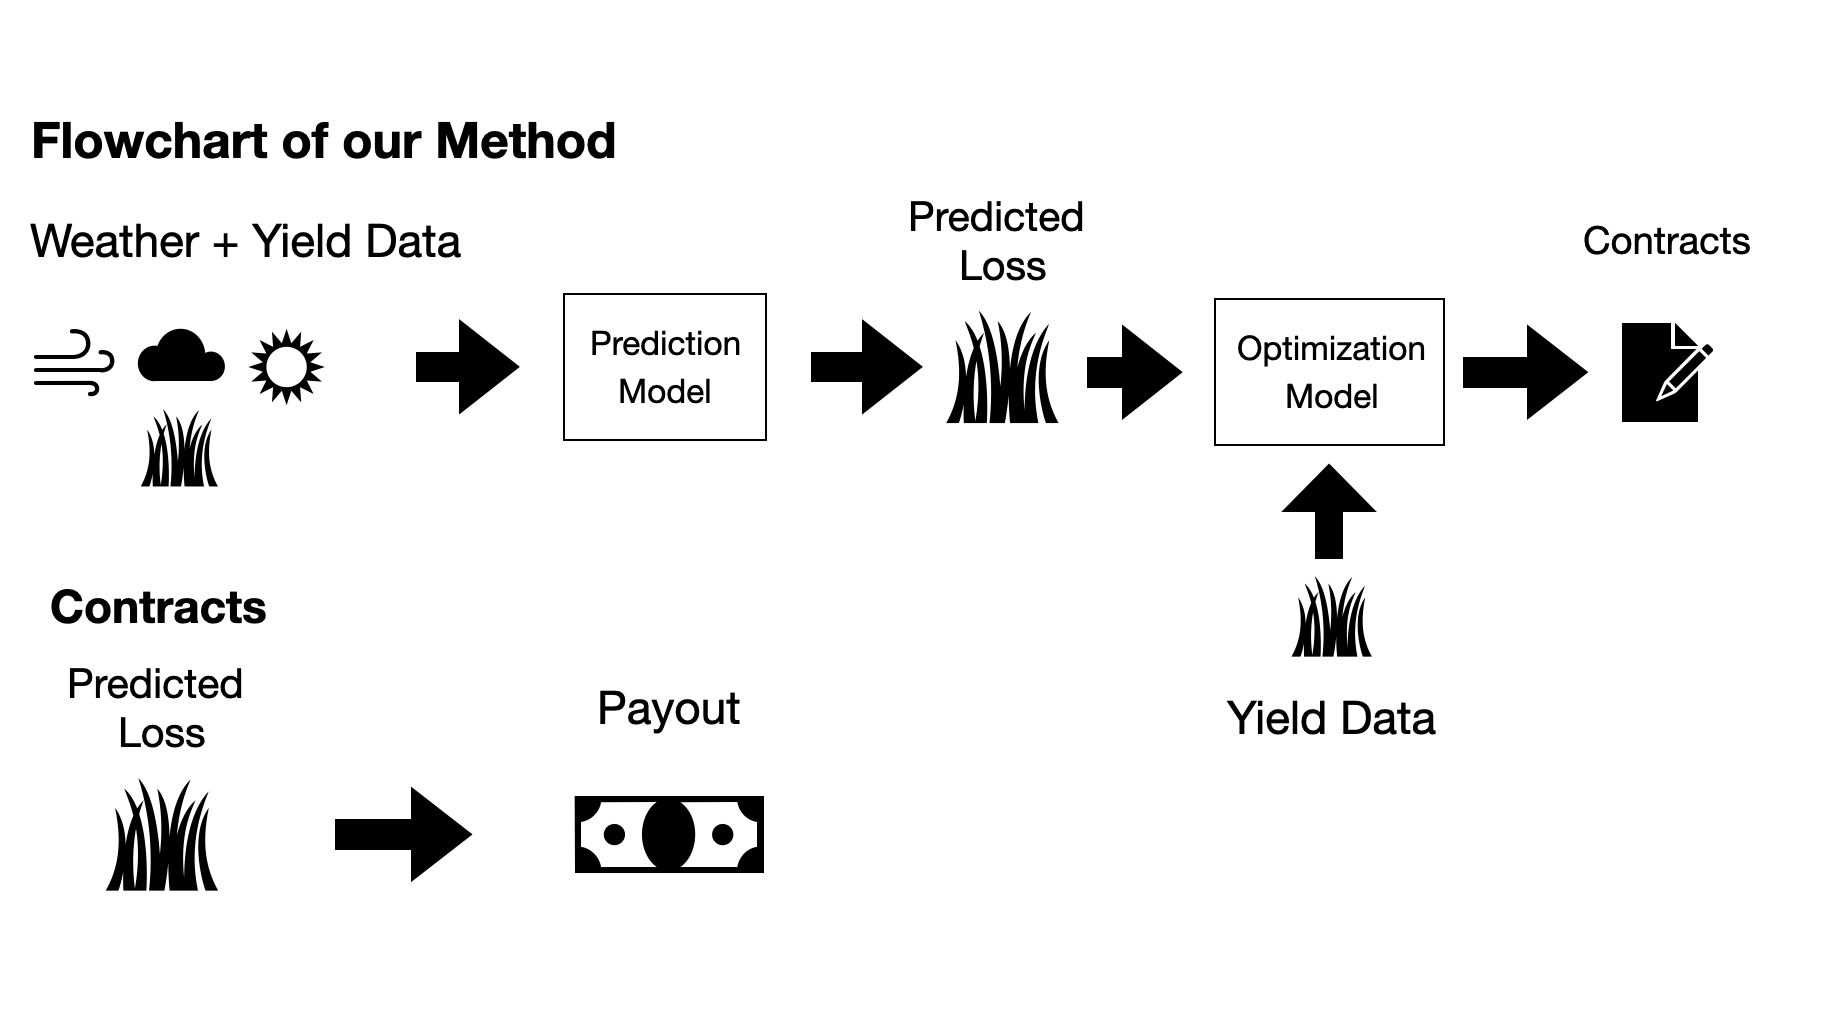
\includegraphics[width=\textwidth]{../../../output/figures/Our Method Flowchart.png}
    \end{figure}
\end{frame}

\subsection{Model}
\begin{frame}{Model}
    Farmers start with wealth, $w_0$ and experience loss $\ell$. There is an index insurance contract $I$, that is determined by a $p$ dimensional vector of indices $\theta = (\theta_1,...,\theta_p)$. Premium for contract $I$ is $\pi(I)$. Farmer wealth is: 
    \begin{align*}
       & w = w_0 -\ell + I(\theta) -\pi(I)\\
       & \pi = \Pi(I)\\
    \end{align*}
    Here, $\Pi$ is the premium principle that is used to determine the insurance contract's price. There are several premium principles that are common in the actuarial literature, and our method is compatible with most of them:
    \begin{table}[h!]
        \centering
        \begin{tabular}{ll}
        Description & Definition \\ \hline
        Expected value       & $(1+\alpha)\mathbb{E}[I]$           \\
        Standard deviation   & $\mathbb{E}[I] + \alpha \sigma(I)$       \\
        Variance             & $\mathbb{E}[I] + \alpha \sigma^2(I)$      \\
        Exponential          & $\frac{1}{\alpha} \log \mathbb{E}[e^{\alpha I}]$    \\
        Dutch                &  $\mathbb{E}[I] + \beta \mathbb{E}[(I-\alpha \mathbb{E}[I])_+]$                   \\ \hline
        \end{tabular}
        \end{table}
\end{frame}

\begin{frame}{Idealized Model}
\label{ideal-model}
\begin{align}
    \max_{a,b,\pi, K}  & \quad \mathbb{E} \left [ U\left ( w_0 - \ell - \pi + I(\theta) \right ) \right ] \label{cons-objective}\\
    \text{s.t.} & \quad I(\theta) =  \min \left \{\max \left \{0,a\hat{\ell}(\theta) + b \right \}, 1 \right \}\label{cons-contract}\\
    & \quad \pi = \mathbb{E}\left [ I(\theta) \right ] + c_{\kappa} \left[ {\sf CVaR}_{1-\epsilon_K}\left ( I(\theta)\right )  - \mathbb{E}[I(\theta)]  \right] \\
    & \quad \underline{f} \leq \mathbb{P}\left ( I(\theta) > 0 \right ) \leq \overline{f} \label{cons-frequency}\\
    &\quad \pi \leq \overline{\pi}.\label{cons-capital}
\end{align}
\end{frame}

\begin{frame}{Convex Relaxation}

    We use the following convex and concave relaxations of $I(\theta)$: 
    \[
    \overline{I(\theta)} \triangleq\ \max \left \{ 0,a\hat{\ell}(\theta) + b\right \},\ \ \ \ 
    \underline{I(\theta)} \triangleq\ \min \{ a\hat{\ell}(\theta) + b,1 \}.
    \]
    Note that $\overline{I(\theta)}$ is convex in $\hat{\ell}(\theta)$, $\underline{I(\theta)}$ is concave in $\hat{\ell}(\theta)$, and
    \begin{align*}
    \underline{I(\theta)} \leq\ I(\theta) \leq\ \overline{I(\theta)}.
    \end{align*}
 We replace $I(\theta)$ in Problem \eqref{cons-objective} with either $\overline{I(\theta)}$ or $\underline{I(\theta)}$ where necessary to obtain a conservative and convex relaxation. 
% \hyperlink{ideal-model}{\beamerbutton{Idealized model}}\\
% \hyperlink{convex-approx}{\beamerbutton{Convex approximations}}
\end{frame}

\begin{frame}{Convex Relaxation}
    \begin{align}
        \max_{a,b,K,\pi} &\quad \mathbb{E} \left [  U\left(w_0 - \ell - \pi  +  \underline{I(\theta)} \right) \right ]\label{eq-06}\\
        \text{s.t.} & \quad \overline{I(\theta)} = \max \left \{0,a\hat{\ell}(\theta) + b \right \} \nonumber\\
        & \quad \underline{I(\theta)} = \min \left \{a\hat{\ell}(\theta)+b,1 \right \} \nonumber\\
        & \quad \pi = \left (1-c_{\kappa} \right ) \mathbb{E} \left [ \overline{I(\theta)} \right ] + c_{\kappa} {\sf CVaR}_{1-\epsilon_K} \left( \overline{I(\theta)} \right) \label{eq-41}\\
        & \quad a \hat{F}^{-1}(\overline{f}) \leq b \leq a\hat{F}^{-1}(\underline{f})\\
        & \quad \pi \leq \overline{\pi} \nonumber.
  \end{align}
    
\end{frame}

\section{Evaluation}
\begin{frame}[noframenumbering, plain]
    \frametitle{Content}
    \tableofcontents[currentsection]
  \end{frame}
\subsection{Data}
\begin{frame}{Data}
    Used two main data sources
    \begin{itemize}
        \setlength\itemsep{2em}
        \item Illinois annual corn yield data from the National Agricultural Statistics Service (NASS). Data is available at the county level from 1925-2022. 84 counties. 
        \item Weather data from the PRISM climate group. Has monthly data on several weather variables (temperature, precipitation, etc). Available 1895-present.
    \end{itemize}
\end{frame}

\subsection{Procedure}
\begin{frame}
    \begin{itemize}
        \setlength\itemsep{2em}
        \item We use a 70/15/15 train/val/test split. Data is kept in chronological order. Training data has older years and test data has the newest years. 
        \item We use the training and validation data to design the contracts using both methods, apply the contracts to farmers in the test set, and compute performance metrics. 
        \item We used a data shortening exercise to evaluate how the performance of both methods changed as more data became available. 
    \end{itemize}
\end{frame}

\subsection*{Illinois Results}
\begin{frame}{Illinois Results: Short Datasets (Less than 40 years of data)}
    \begin{table}
        \begin{tabular}{lrrr}
            \toprule
                  Method &  DeltaCE &  Premium &  Insurer Cost \\
            \midrule
            Our Method &     0.05 &    62.49 &             68,890 \\
               Kenya ILRB &     0.04 &   113.96 &            122,196 \\
                 Chen uc &     0.05 &    60.69 &            52,303 \\
            \bottomrule
            \end{tabular}
    \end{table}
\end{frame}

\begin{frame}{Illinois Results: Long Datasets (More than 40 years of data)}
    \begin{table}
        \begin{tabular}{lrrr}
            \toprule
                  Method &  DeltaCE &  Premium &  Insurer Cost \\
            \midrule
            Our Method &     0.04 &    41.75 &             45,494 \\
               Kenya ILRB &     0.02 &   105.53 &            116,728 \\
                 Chen uc &     0.05 &    50.06 &            44,822 \\
            \bottomrule
            \end{tabular}
    \end{table}
\end{frame}

\section{Multiple Zone Model}
\begin{frame}
    \begin{itemize}
        \setlength\itemsep{2em}
        \item Correlation of losses in the portfolio are important for insurers. 
        \item We use a portfolio approach for premium pricing. 
        \item We incorporate this premium pricing into the optmization model. 
    \end{itemize}
\end{frame}

\begin{frame}{Multiple Zone Model}
    \begin{itemize}
        \setlength\itemsep{2em}
        \item Our method can be extended to design the contracts of multiple zones simultaneously. 
        \item This allows it to take into account the correlation between the insured zones, allowing it to manage risk better. 
    \end{itemize}
    \end{frame}
    
    \begin{frame}{Multiple Zone Model}
        \begin{align}
            \max_{a,b,K,\pi} &\quad \mathbb{E}\left [ \sum_z U\left ( w_{0,z} -\ell_z^j -\pi_z + I_z(\theta^j_z) \right ) \right ]\label{eq-33}\\
            \text{s.t.} &\quad \pi_z  = \mathbb{E}\left [ \overline{I_z(\theta_z)} \right ] + \frac{c_{\kappa}}{\sum_z s_z}  K\\
            &\quad K = {\sf CVaR}_{1-\epsilon_K} \left ( \sum_z s_z\overline{I_z(\theta_z)} \right ) - \mathbb{E}\left [ \sum_{z} s_{z}\underline{I_{z}(\theta_{z'})} \right ] \label{eq-32}\\
            % & \quad a_z\hat{\ell_{z}^{\underline{f}}} \leq b_z \leq a_z\hat{\ell_{z}^{\overline{f}}}\\
            &\quad \overline{I_z(\theta_z)} = \max \left \{0,a_z\hat{\ell_z}(\theta_z) + b_z \right \} \nonumber\\
            &\quad\underline{I_z(\theta_z)} = \min \left \{a_z\hat{\ell_z}(\theta_z)+b_z,1 \right \} \nonumber\\
            &\quad\pi_z \leq \overline{\pi_z} \nonumber.
          \end{align}
    \end{frame}

\subsection{Results}
\begin{frame}{Overview}
    \begin{itemize}
        \item We evaluate our multiple zone model using data from Illinois, Indiana, Missouri, and Iowa. We examine the costs of insuring all four zones simultaneously using the three methods. 
        \item Our multiple zone model adjusts contracts based on the correlation between the insured zones. In this case, it leads to contracts that pay out more frequently, but at a lower rate. This reduces the tail risk for the insurer and reduces the amount of capital needed. 
        \item It outperforms Chen's model and the no insurance case consistently, and has lower costs and required capital than the Chen model. 
    \end{itemize}
\end{frame}

\begin{frame}{Midwest Results: Short datasets (Less than 40 years)}
    \begin{table}
        \begin{tabular}{lrrr}
            \toprule
                  Method &  DeltaU &  Insurer Cost &  Required Capital \\
            \midrule
            Our Method &   0.04 &     150,414 &           $6.6\%$ \\
               Kenya ILRB &   0.06 &     397,474 &          $4.4\%$ \\
                 Chen uc &    -0.09 &     159,928 &          $12\%$ \\
            \bottomrule
            \end{tabular}
    \end{table}
\end{frame}

\begin{frame}{Midwest Results: Long datasets (More than 40 years)}
    \begin{table}
        \begin{tabular}{lrrr}
            \toprule
                  Method &  DeltaU &  Insurer Cost &  Required Capital \\
            \midrule
            Our Method &   0.03 &      99,769 &           $5.6\%$ \\
               Kenya ILRB &   0.02 &     389,678 &          $4.3\%$ \\
                 Chen uc &   0.00 &     141,651 &          $8.6\%$ \\
            \bottomrule
            \end{tabular}
    \end{table}
\end{frame}

\section{Evaluation: Thai Data}
\begin{frame}{Data Description}
    \begin{itemize}
        \setlength\itemsep{2em}
        \item We use Tambon level loss data from the Department of Agricultural Extension and the BAAC 
        \item Weather data from Google Earth Engine, we use rainfall, evapotranspiration, and temperature. 
    \end{itemize}
\end{frame}


\begin{frame}{Results: Single Zone}
    
\end{frame}

\begin{frame}{Results: Multiple Zones}
\end{frame}

\begin{frame}{Midwest: Required Capital}
    \begin{figure}
        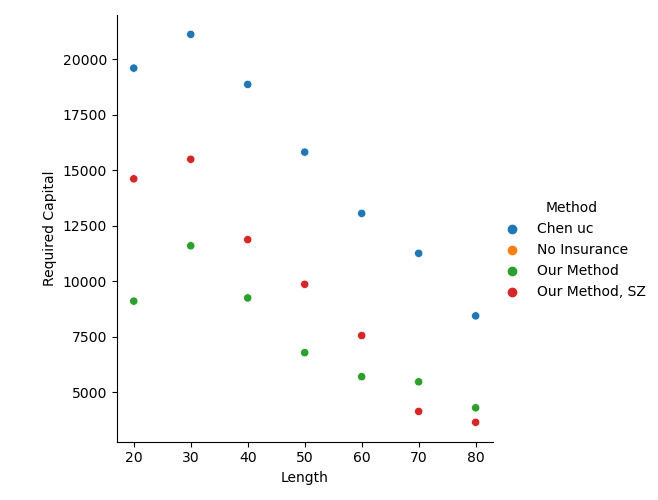
\includegraphics[width=0.75\textwidth]{../../../output/figures/Midwest Evaluation/Midwest_Required Capital_Length.png}
    \end{figure}
\end{frame}

\subsection*{Illinois Results}
\begin{frame}{Illinois: Utility}
    \begin{figure}
        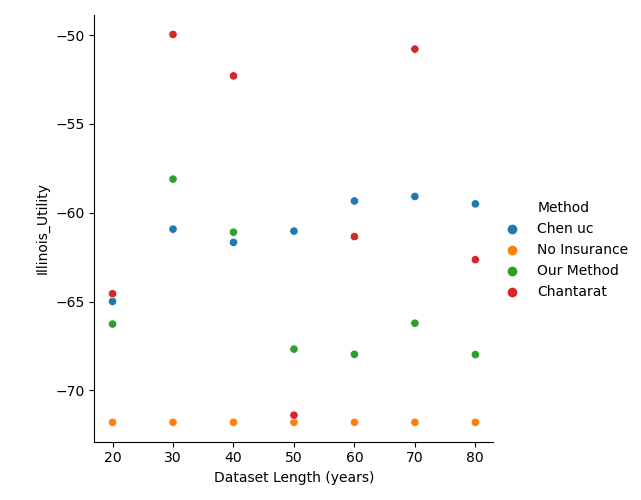
\includegraphics[width=0.75\textwidth]{../../../output/figures/Midwest Evaluation/Illinois_Utility_Length.png}
    \end{figure}
\end{frame}

\subsection*{Iowa Results}
\begin{frame}{Iowa: Utility}
    \begin{figure}
        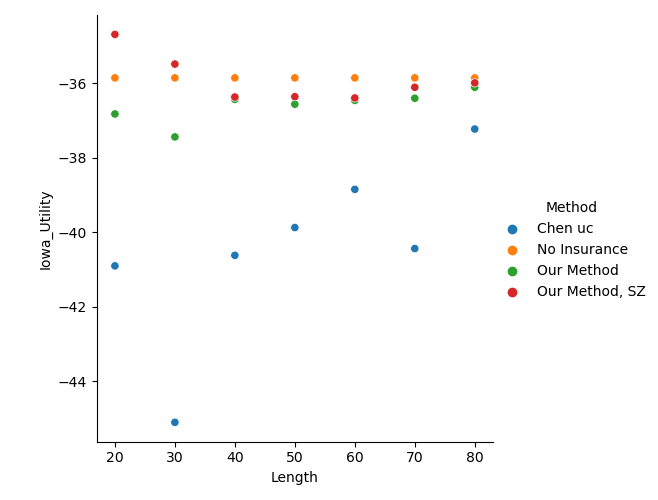
\includegraphics[width=0.75\textwidth]{../../../output/figures/Midwest Evaluation/Iowa_Utility_Length.png}
    \end{figure}
\end{frame}

\subsection*{Missouri Results}
\begin{frame}{Missouri Utility}
    \begin{figure}
        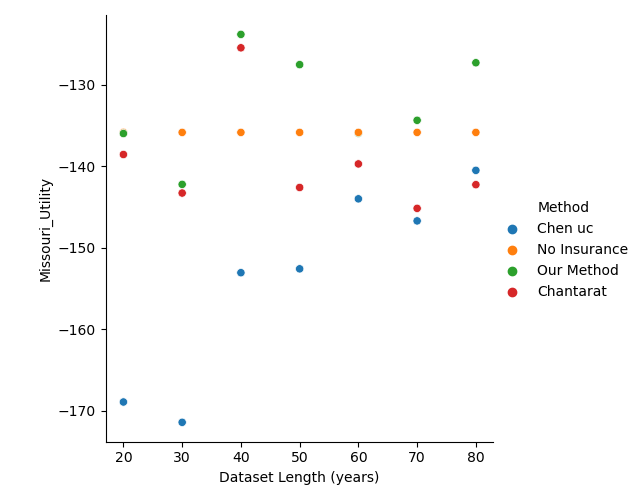
\includegraphics[width=0.75\textwidth]{../../../output/figures/Midwest Evaluation/Missouri_Utility_Length.png}
    \end{figure}
\end{frame}

\subsection*{Indiana Results}
\begin{frame}{Indiana Utility}
    \begin{figure}
        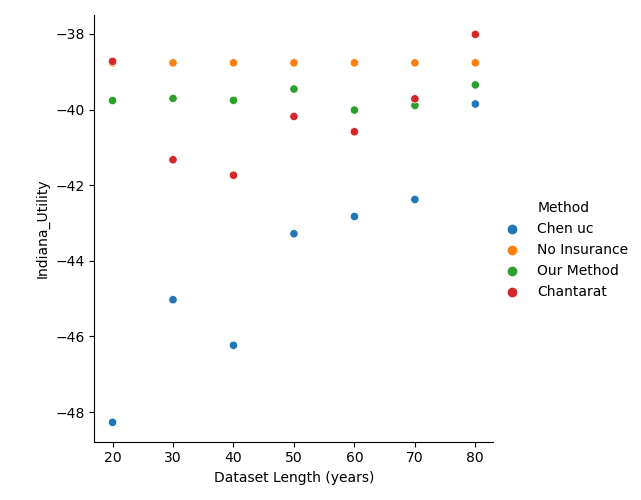
\includegraphics[width=0.75\textwidth]{../../../output/figures/Midwest Evaluation/Indiana_Utility_Length.png}
    \end{figure}
\end{frame}


\section*{Implementation Details}
\begin{frame}{Loss Definition}
    From what I can tell from the replication files, they seem to define loss in every year as: 
    \begin{align*}
        \ell_{st} &= R^*_s - R_{st}
    \end{align*}

    where $R^*_s$ is the maximum revenue observed in state $s$ across all time periods, and $R_{st}$ is the revenue in state $s$ at time $t$. 
\end{frame}

\begin{frame}{Initial wealth}
    According to the paper, they set $w_0 = 389$. However, in the replication files, they set it to be $w_0 = 813 - 504 + 389$. According to the comments, $504$ is the fixed cost of operating a farm, and there are no comments regarding the $813$, I'm assuming it corresponds to $R^*$. 
\end{frame}

\begin{frame}{Detrending}
    \begin{itemize}
        \item According to the paper, they detrend the county level yield data using a 2nd order polynomial fit with a ``robust'' regression method, but they don't specify what they use, and it's not in the replication files. They also don't specify if they remove the trend using additive or multiplicative decomposition model. Using an additive decomposition model yielded the most similar losses to what they provide in the replication files. 
        \item There are a couple of papers showing that using locally weighted regression to detrend works better. 
    \end{itemize}
    
\end{frame}

\section*{Questions}
\begin{frame}{Questions}
    \begin{itemize}
        \item Would it make sense to define loss as deviation from historical average? Allowing it to be positive in some years? In other words, we would first adjust all of the yield data to 2020 levels and then calculate the historical average. The loss in each year would be the deviation from this historical average. 
        \item Should I simply follow their lead on detrending? Or should I try to improve on it?
        \item Do you think it's necessary to show results with both definitions of the premium?
        \item Do you think subsidy vs lump sum results would be interesting?
    \end{itemize}
\end{frame}

\section*{Chen Premium Results}
\subsection*{Illinois Results}
\begin{frame}{Their Defn of Premium: Illinois Utility}
    \begin{figure}
        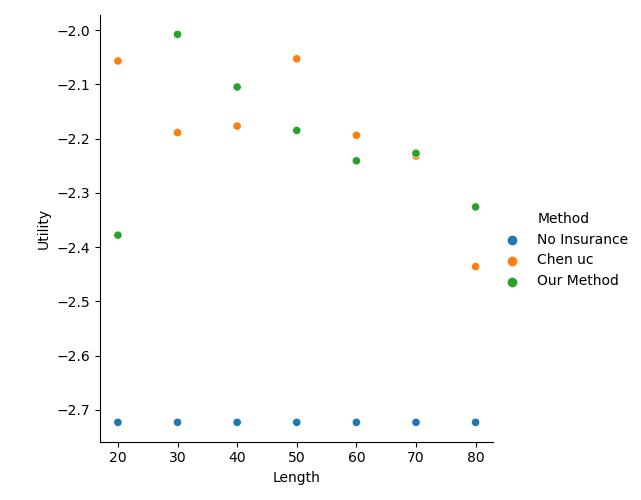
\includegraphics[width=0.75\textwidth]{../../../output/figures/Chen Premium/Illinois_Utility_Length_ml1241.png}
    \end{figure}
\end{frame}

\subsection*{Iowa Results}
\begin{frame}{Their Defn of Premium: Iowa Utility}
    \begin{figure}
        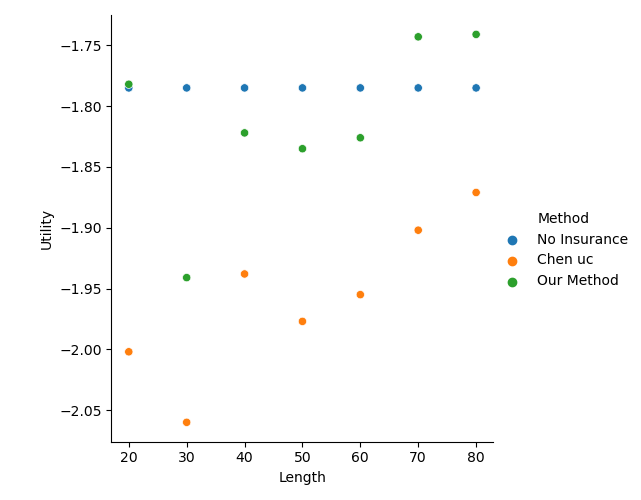
\includegraphics[width=0.75\textwidth]{../../../output/figures/Chen Premium/Iowa_Utility_Length_ml1241.png}
    \end{figure}
\end{frame}

\subsection*{Missouri Results}
\begin{frame}{Their Defn of Premium: Missouri Utility}
    \begin{figure}
        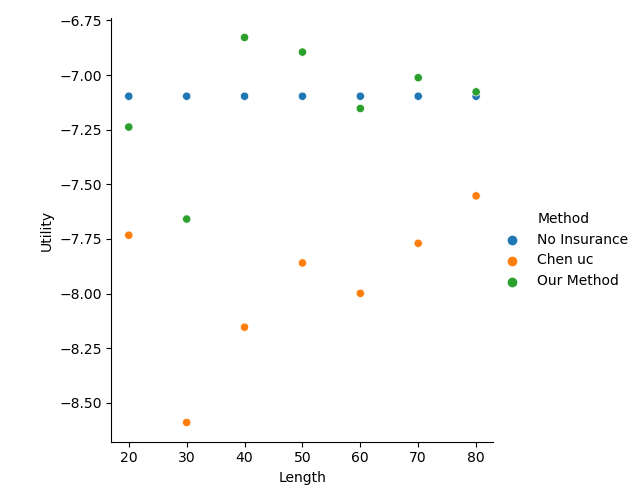
\includegraphics[width=0.75\textwidth]{../../../output/figures/Chen Premium/Missouri_Utility_Length_ml1241.png}
    \end{figure}
\end{frame}

\subsection*{Indiana Results}
\begin{frame}{Their Defn of Premium: Indiana Utility}
    \begin{figure}
        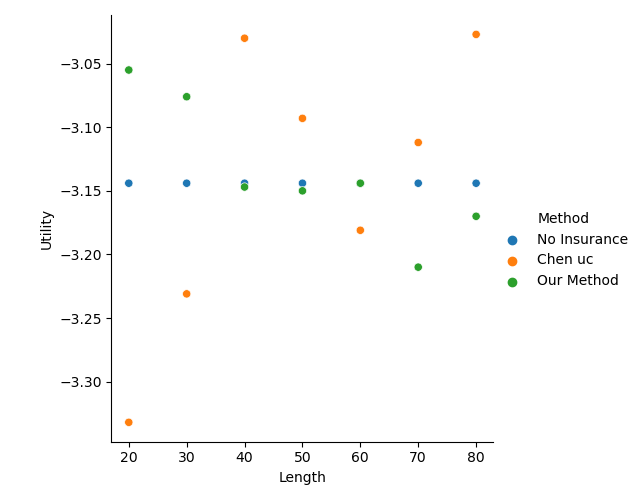
\includegraphics[width=0.75\textwidth]{../../../output/figures/Chen Premium/Indiana_Utility_Length_ml1241.png}
    \end{figure}
\end{frame}



% \section{Conclusion and Next Steps}
% \subsection{Conclusions}
% \begin{frame}{Conclusions}
%     \begin{itemize}
%     \setlength\itemsep{2em}
%         \item The contracts designed by our model are able to offer better protection at a similar costs, or comparable protection at lower costs than the baseline method. 
%         \item It outperforms the baseline when the prediction model is incorrectly specified and on the Kenyan pastoralist data. 
%         \item Our method is more cost effective because it takes into account spatial correlations between  areas and the costs of capital requirements. Thus, the model makes better trade offs between costs and coverage than the baseline method. 
        
%     \end{itemize}
% \end{frame}

% \subsection{Next Steps}
% \begin{frame}{Next Steps}
% \begin{itemize}
% \setlength\itemsep{2em}
%     \item We are working with practitioners to improve the model and possibly test it in practice.
%     \item We are working with the Bank of Thailand on the implementation of their satellite-based index insurance program. 
%     \item We are also talking to the International Research Institute for Climate and Society at Columbia, they have worked on the implementation of numerous index insurance programs in Africa.   
% \end{itemize}
% \end{frame}

\begin{frame}[noframenumbering, plain]{References}
\printbibliography
\end{frame}

\begin{frame}[noframenumbering, plain]{Idealized CVaR Model}
% \label{ideal-model}
\begin{itemize}
    \item \textbf{Objective:} conditional value at risk of the farmers' loss net of insurance.
    \item  \textbf{Constraint 1:} piecewise linear structure of the contract. 
    \item \textbf{Constraint 2:} budget constraint.
    \item \textbf{Constraint 3:} definition of required capital.
\end{itemize}
 
\begin{align}
        \min_{a,b,\pi, K}  & \quad CVaR_{1-\epsilon}\left ( \ell - I(\theta) \right ) \notag\\
        \text{s.t.   }I(\theta) &= \min \{ (a\hat{\ell}(\theta) + b)^+,P \} \\
        \mathbb{E}\left [ I(\theta) \right ] &+ c_{\kappa} K \leq B \\
        K &= \left( CVaR_{1-\epsilon}\left ( I(\theta) \right ) - \mathbb{E}[I(\theta)] \right) \label{cons-budget}
    \end{align}
\end{frame}

\begin{frame}[noframenumbering, plain]{The problem is non-convex, so we need convex approximations}
\label{convex-approx}
We use the following approximations of $I(\theta)$ to make the problem convex: 
\begin{align*}
    \overline{I(\theta)} &\triangleq \max \left \{ 0,a\hat{\ell}(\theta) + b\right \} \\
    \underline{I(\theta)} &\triangleq \min \{ a\hat{\ell}(\theta) + b,K \}
\end{align*}
\begin{itemize}
    \item Note that $\overline{I(\theta)} \geq I(\theta)$ and $\overline{I(\theta)}$ is convex. Conversely, $\underline{I(\theta)} \leq I(\theta)$ and $\underline{I(\theta)}$ is concave. 
    \item We replace $I(\theta)$ with either $\overline{I(\theta)}$ or $\underline{I(\theta)}$ where necessary to obtain conservative and convex approximations. 
    \item We also need approximations or proxies for $E[I(\theta)]$ in constraint . We use $\pi_{SQ} = E[I_{SQ}(\theta)]$, where $I_{SQ}$ is the contract designed using the status quo method, as a proxy for $E[I(\theta)]$ in constraint .
\end{itemize}
\end{frame}



\end{document}